\chapter{Distribution and Growth} \label{chapter-distribution}

\epigraph{A large body of literature documents the existence of agglomeration economies in developed economies (see Rosenthal and Strange 2004 for a review). The main conclusion of this literature is the finding of scale economies of 3–8 percent (that is, a 10 percent increase in the size of an activity in a city raises productivity in this activity by 0.3– 0.8 percent).}{Gilles Duranton \cite{durantonAreCitiesEngines2009}} 


%Cities are the engines of economic growth (Jacobs, 1969; Bairoch, 1988). It is in cities that a large share of the innova- tions and entrepreneurship takes place that fosters economic growth in the long run. Spontaneous Orders and the Emergence of Economically Powerful Cities. JOHANNA PALMBERG

A growing body of research on urban scaling has demonstrated increasing returns to population. In our chapter on growth theory we showed that neoclassical growth theory associated these increasing returns to scale at the urban or national level with increasing effective human capital, which grows faster than the labour supply as a result of increased education or agglomeration effects. The two lines of research have settled on what might be termed a  common ``stylized  fact'': population and output are related according to 
\begin{equation}
    Y=AN^\beta,\qquad \beta>1 \label{equation-the-fact}
\end{equation}
% can be expressed as Y (\lambda N)~Z(\lambda,N)Y (N). When the scale factor Z depends only on \lambda, i.e. Z(\lambda,N)~Z(\lambda), equation (2) can be solved uniquely to give the scale-invariant result of equation (1), with Z(l\lambda)~\lambda^\beta.

Equation~\ref{equation-the-fact}  is a high-level generalization -- a ``coarse'' grained model.
% There's a distinction between coarse grained and fine grained models. 
A core problem in modelling is the tradeoff between computational tractibility and representing details. 
Coarse grained models must capture the stylized facts.
% where the model is insenstitive to the details, you really want a representation that's small that captures the big pattern. 
When you move to getting the details of the model, you know you have a model that tracks the observable. 

\cite{GET_TerrysDissertation, GET_PaulsBook}


Empirical estimates of $\beta$ vary considerably\cite{rosenthalEvidenceNatureSources2004}\cite{bettencourtIntroductionUrbanScience2021} \cite{loboUrbanScalingProduction2013}. 
McCoskey and Kao \cite{mccoskeyPanelDataInvestigation}show that  the impact of urbanization on growth varies greatly across countries in different countries.
The World Bank (2016) reported that every 1\% growth in urban population correlates with an increase in GDP per capita by 13\%, 10\%, and 7\% in India, China, and Thailand, respectively.  However, Indonesia realizes only 4\% GDP growth for every 1\% increase. \cite{haryantotriRelationshipUrbanizationEducation2021}. The literature has not yet offered an explanation  of the variation.\cite{loboUrbanScalingProduction2013}.

% REFERENCES to shcick from LOBO et al:
%18. Carlino GA (1979) Increasing returns to scale in metropolitan manufacturing. J Reg Sci 19: 343–351. 
% % 19. Moomaw RL (1988) Agglomeration economies: localization or urbanization? Urban Stud 25: 150–161. 
% 20. Beaudry C, Schiffauerova A (2009) Who’s right, Marshall or Jacobs? The localization versus urbanization debate. Res Policy 38: 318–337. 
% 21. Duranton G, Puga D (2004) Micro-foundations of urban agglomeration economies. In: Henderson, J.V Thisse, J.F., editors. Handbook of Regional and Urban Economics 4: 2063–2117. 
% 22. Puga D (2010) The magnitude and causes of agglomeration economies. J Urban Econ 50: 203–219. 
% 23. Knudsen B, Florida R, Stolarick K, Gates G (2008) Density and creativity in U.S. regions. Ann Assoc Am Geogr 98: 461–478. 
% 24. Rauch JE (1993) Productivity gains from geographic concentration of human capital: evidence from cities. J Urban Eco 34: 380–400. 
% 25. Rosenthal SS, Strange WC (2001) The determinants of agglomeration. J Urban Econ 50: 191–229. 
% 26. Segal D (1976) Are there returns to scale in city size? Rev Econ Stat 58: 339350. 
% 27. Shefer D (1973) Localization economies in SMSAs: a production function approach. J Reg Sci 13: 55–64. 
% 28. Sveikauskas L (1975) The productivity of cities. Q J Econ 89: 393–413. 
% 29. Moomaw RL (1981) Productivity and city Size? A critique of the evidence. Quarterly Journal of Economics 96: 675–688.
% 



%  MOVE THISAt the national level, Solaki \cite{solakiRelationshipEducationGDP2013} demonstrates a causal relationship between education and growth, and that tertiary Education should be considered as an exogenous variable.  Empirical results for Bangladesh \cite{islam2007relationship}show evidence of bidirectional causality between education and growth.  At the urban level a study by Glaeser and Saiz \cite{glaeserRiseSkilledCity2003} for the US found that human capital predicted population and productivity growth at the city and metropolitan area level as surely as it predicts income growth at the country level. They specifically found that cities with more educated residents have grown more quickly than comparable cities with less human capital. They find that causation running from growth to education seems to be present only in a handful of declining metropolitan areas, and cannot account for much of the relevant effect. Their evidence supports the view that skills induce urban growth.


The source of the variation is a matter of considerable policy importance, however. If $\beta$ can be affected positively by policy choices, or perhaps negatively by trends such as financialization, governments may be able to significantly increase social wealth and wellbeing.\footnote{Interestingly, the residuals or unexplained components for smaller cities are much larger than for large cities, suggesting that clues about potential policies will be found by examining smaller and mid-sized cities and that potential policy impacts may be greater for these cities.}

\begin{figure}
    \centering
    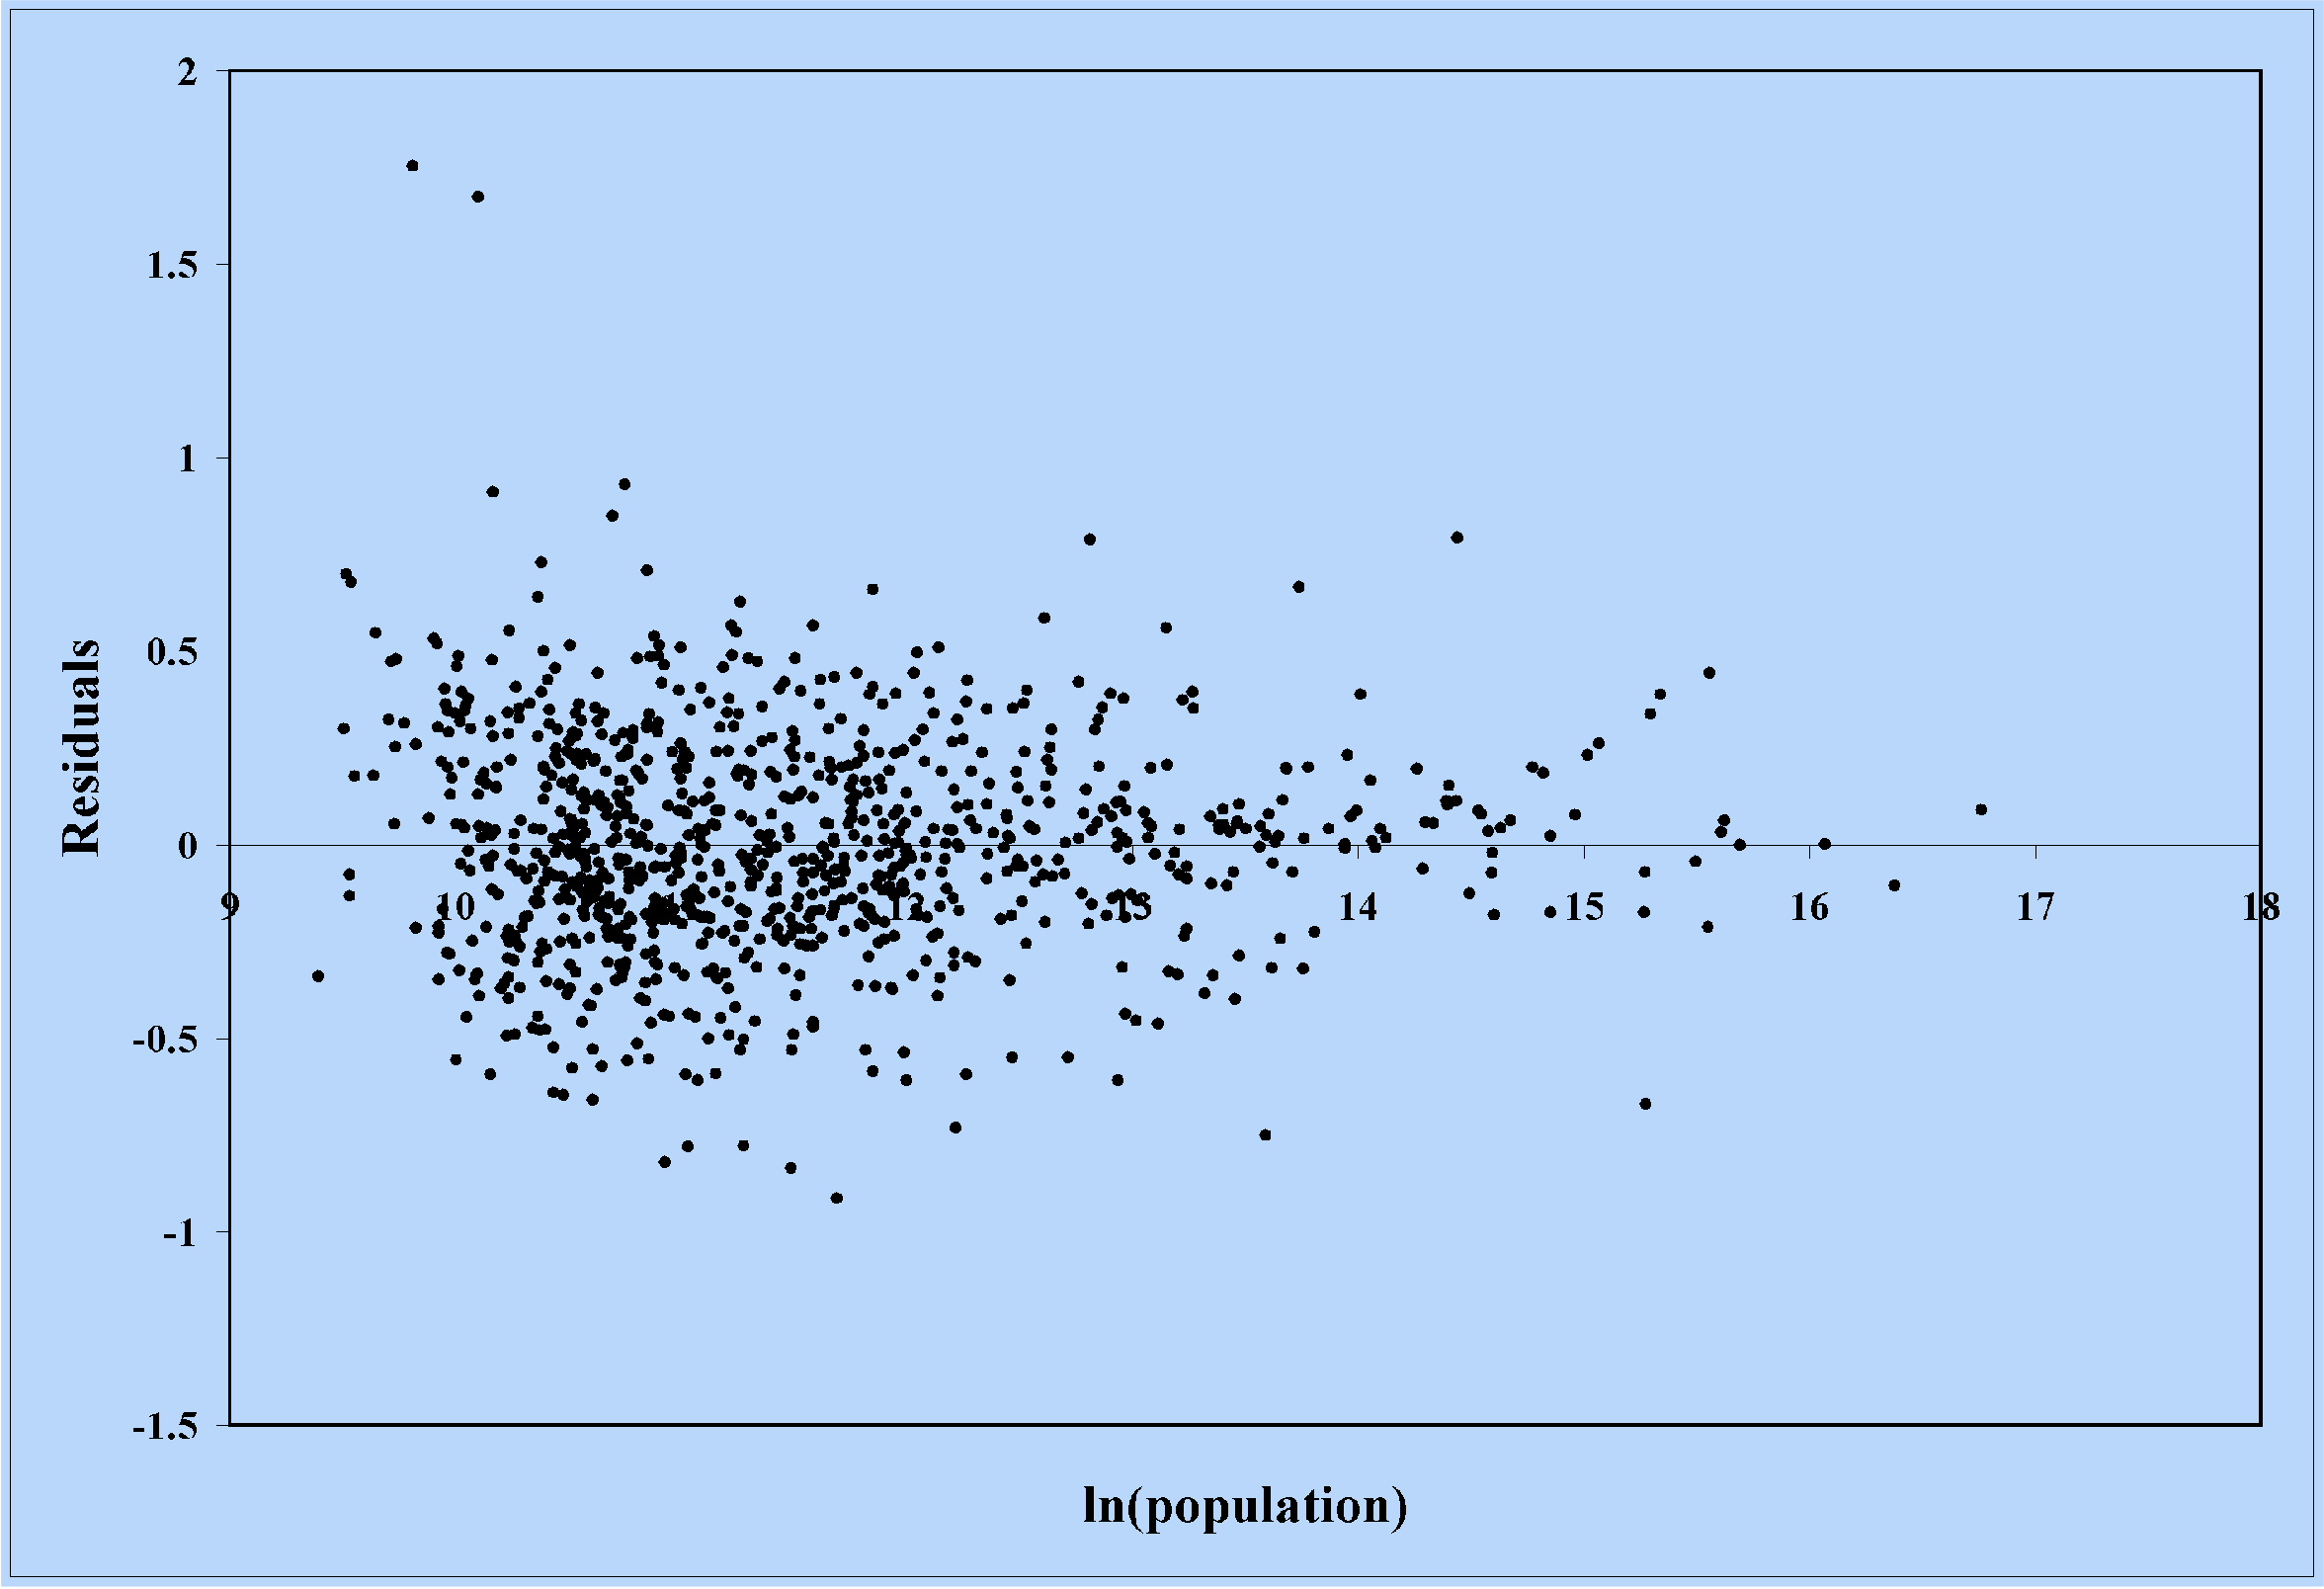
\includegraphics[scale=0.25]{fig/Residuals-Lobo.png}
    \caption{Residuals from regressing ln(total wages) on ln(population) using data for all 943 urban areas of the United States smoothed over the 2009–2011 period. Source: Lobo et al \cite{loboUrbanScalingProduction2013}}
    \label{fig:Residuals-Lobo}
\end{figure}


Equation~\ref{equation-the-fact} is clearly a long-term relationship, because urban productivity can only evolve very slowly. The cross-sectional studies to date are simply not able to identify the long-term effects of all of the variables that might explain the varied results for  $\beta$. The literature has identified many possible channels that affect overall productivity. Neoclassical growth theory, for example, provides one convincing general explanation in terms of human capital, but it does not provide definitive empirical evidence on precisely how the effects of agglomeration are transmitted. Researchers have not settled on which  of the possible influences dominate, what channels they work through, or what policies might improve the transmission of positive effects. These gaps are  not surprising. The literature on urban scaling is relatively new.  Empirical verification will wait on the development of extended time series on urban output.



The analysis of those still unavailable time series, however, will require theoretical models that make $\beta$ depend on policy variables of interest,  In this chapter, we examine a number of potential  links between urban population and productivity that have been proposed, and discuss how we  might incorporate specific policy-relevant linkages into our model.  Our interest is in how financialization might affect cities, and in this chapter specifically on the channels through which financialization might affect the productivity and growth of cities.


%\footnote{Lobo et al are careful not to  claim that there is a causal relation between urban scaling and urban productivity. Causality, they say, stems from the ways in which being embedded inside larger agglomerations fundamentally affects how individuals interact with each other. Such micro-processses have not been demonstrated.}

\section{The transmission puzzle}
We can make a distinction between the myopic marginal productivity curve observed by at the shop floor level and even the firm wide effect of adding a worker. We could go on to consider the slower and distributed effect on closely related firms, which would raise any estimate of marginal product. Expanding our view we  would eventually consider a marginal social productivity of labour that is higher still. 

 In our model the long-term wage is set at the social marginal product of labour, including all external effects on other firms. Wages are set, however, in private markets. It seems likely that the agglomeration effect of adding a worker on the productivity of other workers even within a firm  would be attributed to that worker. For the firm there  would be a lagged, unevenly distributed effect that would appear exogenous, and so would not be
compensated. We may assume therefore that firms do not take the positive externalities into account, implying firms will hire fewer than the optimal number of workers. This seems to be a serious challenge to our decision to model the city relying on Equation~\ref{equation-the-fact} and the  Alonzo-Jacobs cycle.

The scale effects observed, however make it clear that cities do exhibit increasing returns. The argument we have just stated implies  that cities will be chronically inefficient, failing to grow as  much and as quickly as they should because private decision makers fail to take into account the agglomeration externalities. The argument could be correct, but since agglomeration is observed, there must be channels  transmitting at least some of the gains from scaling to the workforce. The possibility that the linkage is slow and partial raises an exciting prospect: it may be possible to improve the  transmission process.

Modelling or even identifying  the actual transmission processes is beyond the scope of this thesis, but our concern with the impact of financialization demands that we at least consider specific channels through which financialization of the housing market might affect the Alonzo-Jacobs cycle. To do this we have identified a range of hypotheses about possible transmission mechanisms and considered how they might be affected by the financialization of the housing market. Our goal is to identify a subset of those hypotheses that may be relevant in policy formation and that therefore may warrant future research.



\section{The Scale-Adjusted Metropolitan Indicator}
 Lobo et al \cite{loboUrbanScalingProduction2013} provide an  analysis that is a useful starting point for search for potential policy levers. They show that Equation~\ref{equation-the-fact} can be written as an explicit function of population size, $N_i$, and specific local deviations, $\xi_i$ that they  call a Scale-Adjusted Metropolitan Indicator (SAMI). The SAMIs they derive depend on local wages and capital costs and they account for the city specific residuals in Figure~\ref{fig:Residuals-Lobo} when $\beta$ is estimated using population alone. 
 
 The model treats Equation~\ref{equation-the-fact} as a production function, as we do in Chapter~\ref{chapter-growth}.  Their preferred form is
 \[Y_i =A N^\beta_ i e^{\xi_i^Y} \eqno  \label{eqn-lobo}\]
    Where $ e^{\xi_i^Y}$ is the city-specific residual for the regression.\footnote{As is usual in this literature, they log Equation~\ref{eqn-lobo} and use linear regression.}   They work backward from this expression to a Cobb-Douglas production function that depends only on labour and capital inputs.\footnote{In Chapter~\ref{chapter-growth} we show how the neoclassical growth theorists , in effect, worked forward form the Cobb-Douglas production function to an expression equivalent to the result form the scale literature.} They conclude that any  variables used to explain the residuals in estimates  of $\beta$ for cities must be expressed in terms of their  contribution to  the wage and capital shares of income or to  the magnitude of wage and capital inputs. 






% \begin{sidewaysfigure}[!ht]
% \caption[]{Impact channels of financialization}
%     \centering
%     \includegraphics[scale=.25]%, angle=90}
%     {fig/impact_channels.png}
%     \label{fig-impact-ch}
% \end{sidewaysfigure}



{\newpage\thispagestyle{empty}
\vspace{-1.5cm}
\begin{figure}
\vspace{-1cm}
\caption{Impact Channels}
% \label{figure-impact-channels}
\begin{adjustwidth}{-0.24\textwidth}{-0.24\textwidth}
    \centering
    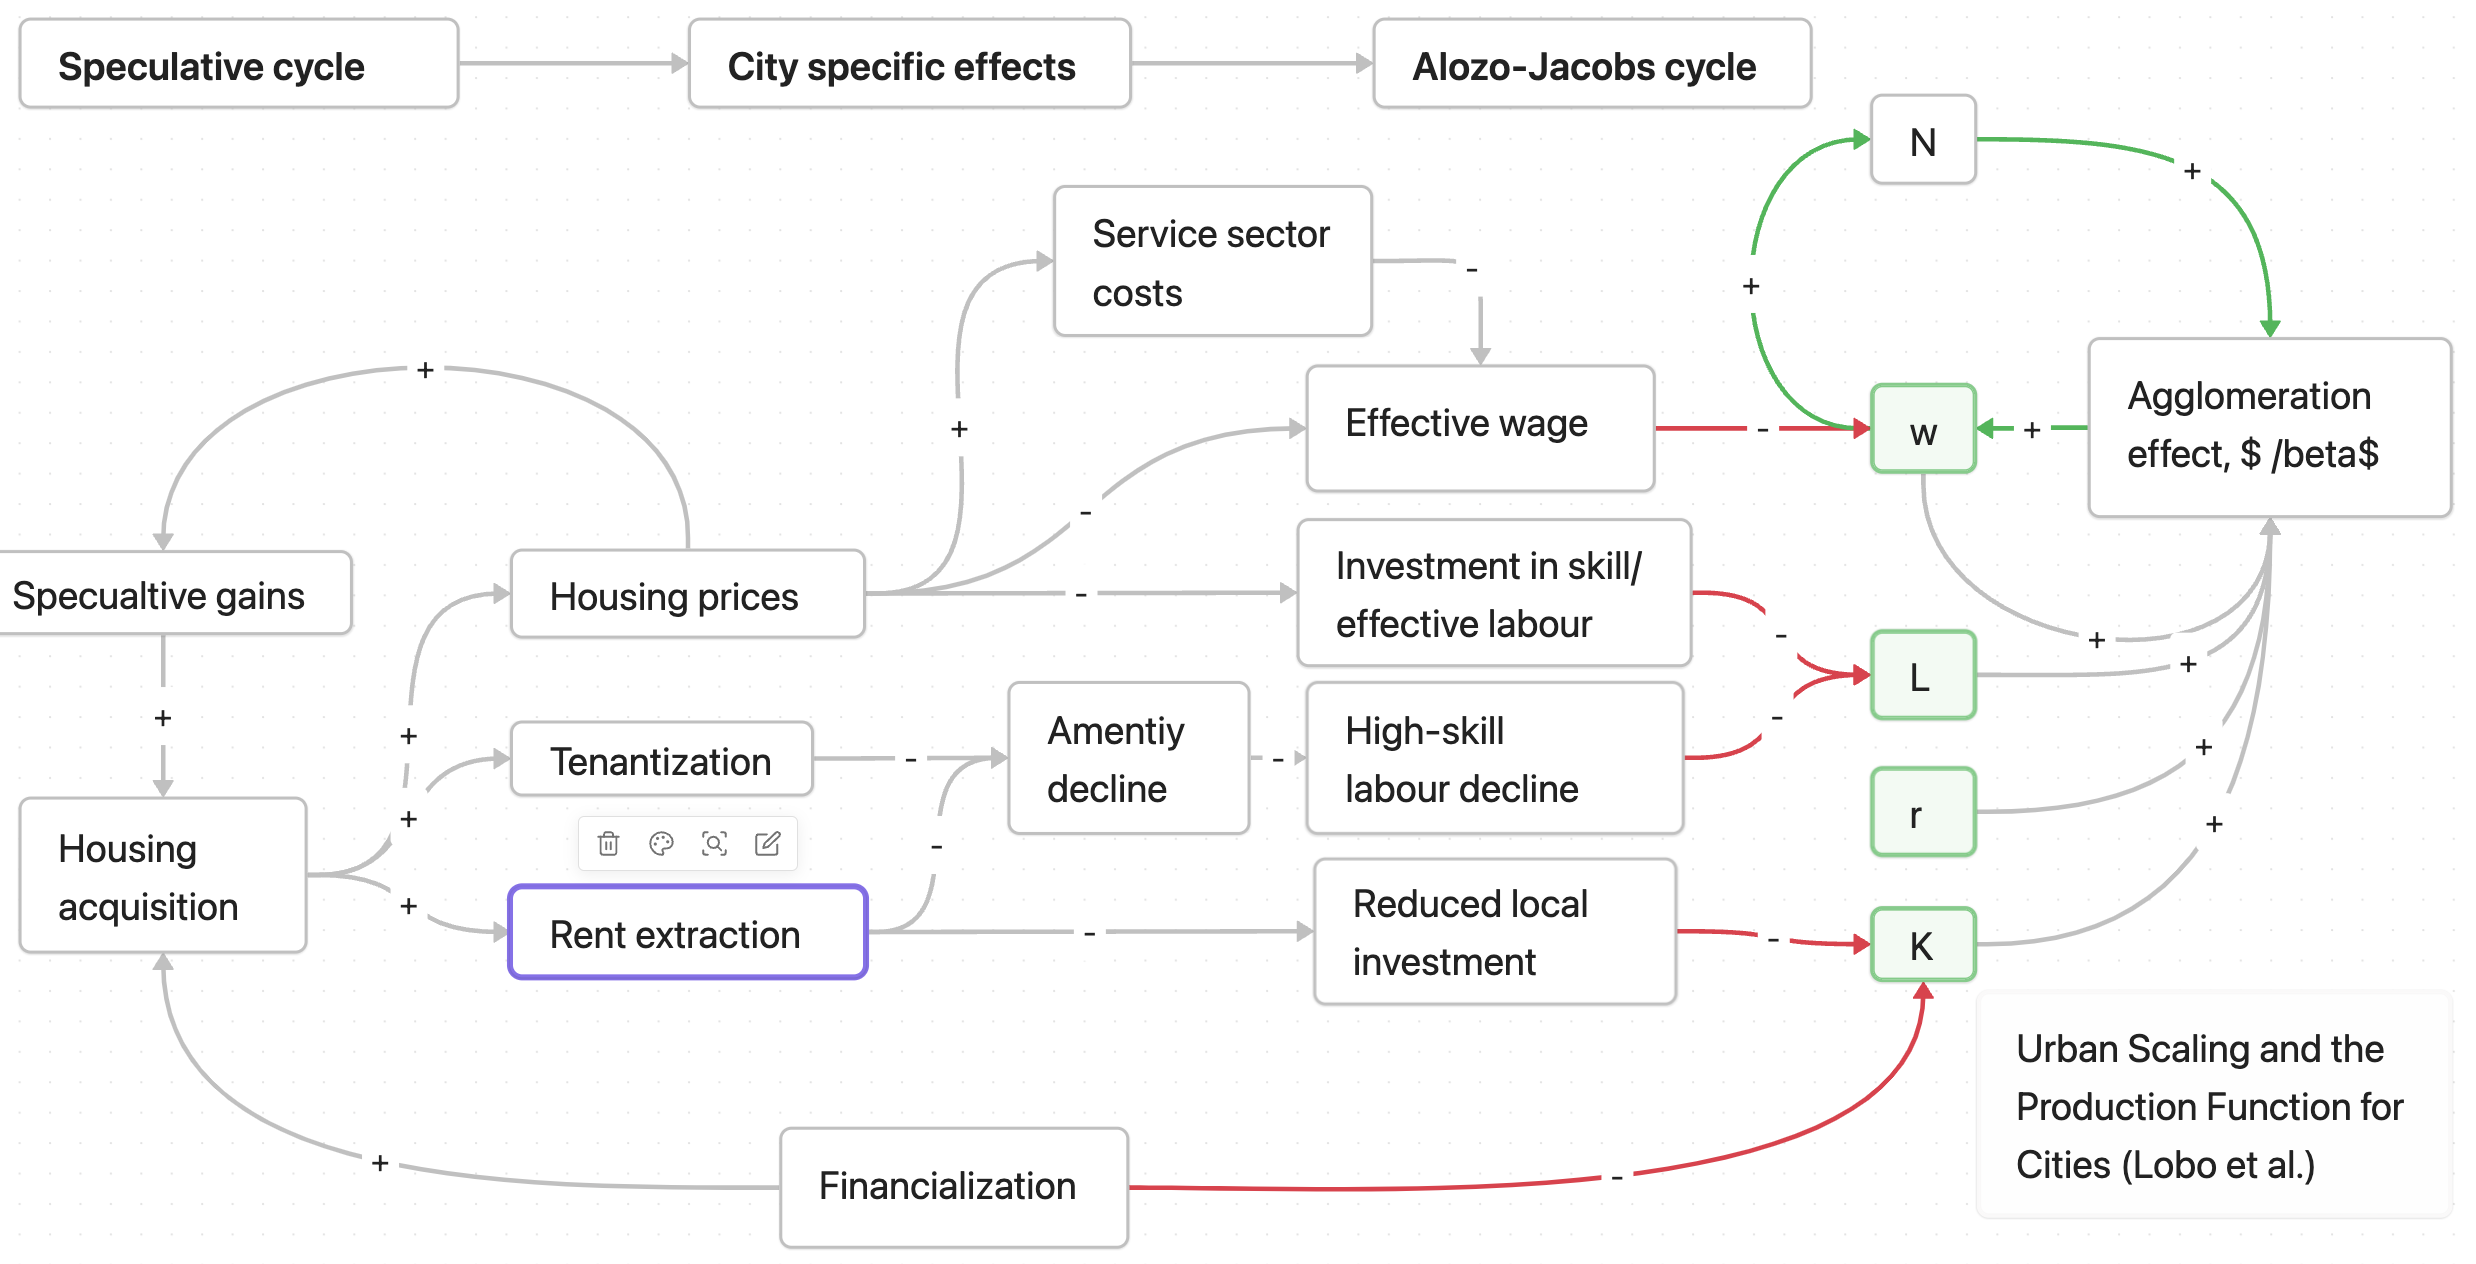
\includegraphics[scale=.45, angle=90]{fig/impact_channels_revised.png}
    \label{fig-impact-channels}
%\pagestyle{headings}
% \usetikzlibrary{positioning}
%\begin{tikzpicture}[remember picture,overlay,shift={(current page.north east)}] \node[anchor=north east,xshift=-1cm,yshift=-1cm]{\includegraphics[width=1cm]{example-image-a}};\end{tikzpicture}
\end{adjustwidth}
\end{figure}
}


% \begin{figure}[!ht]
%     \centering
% %    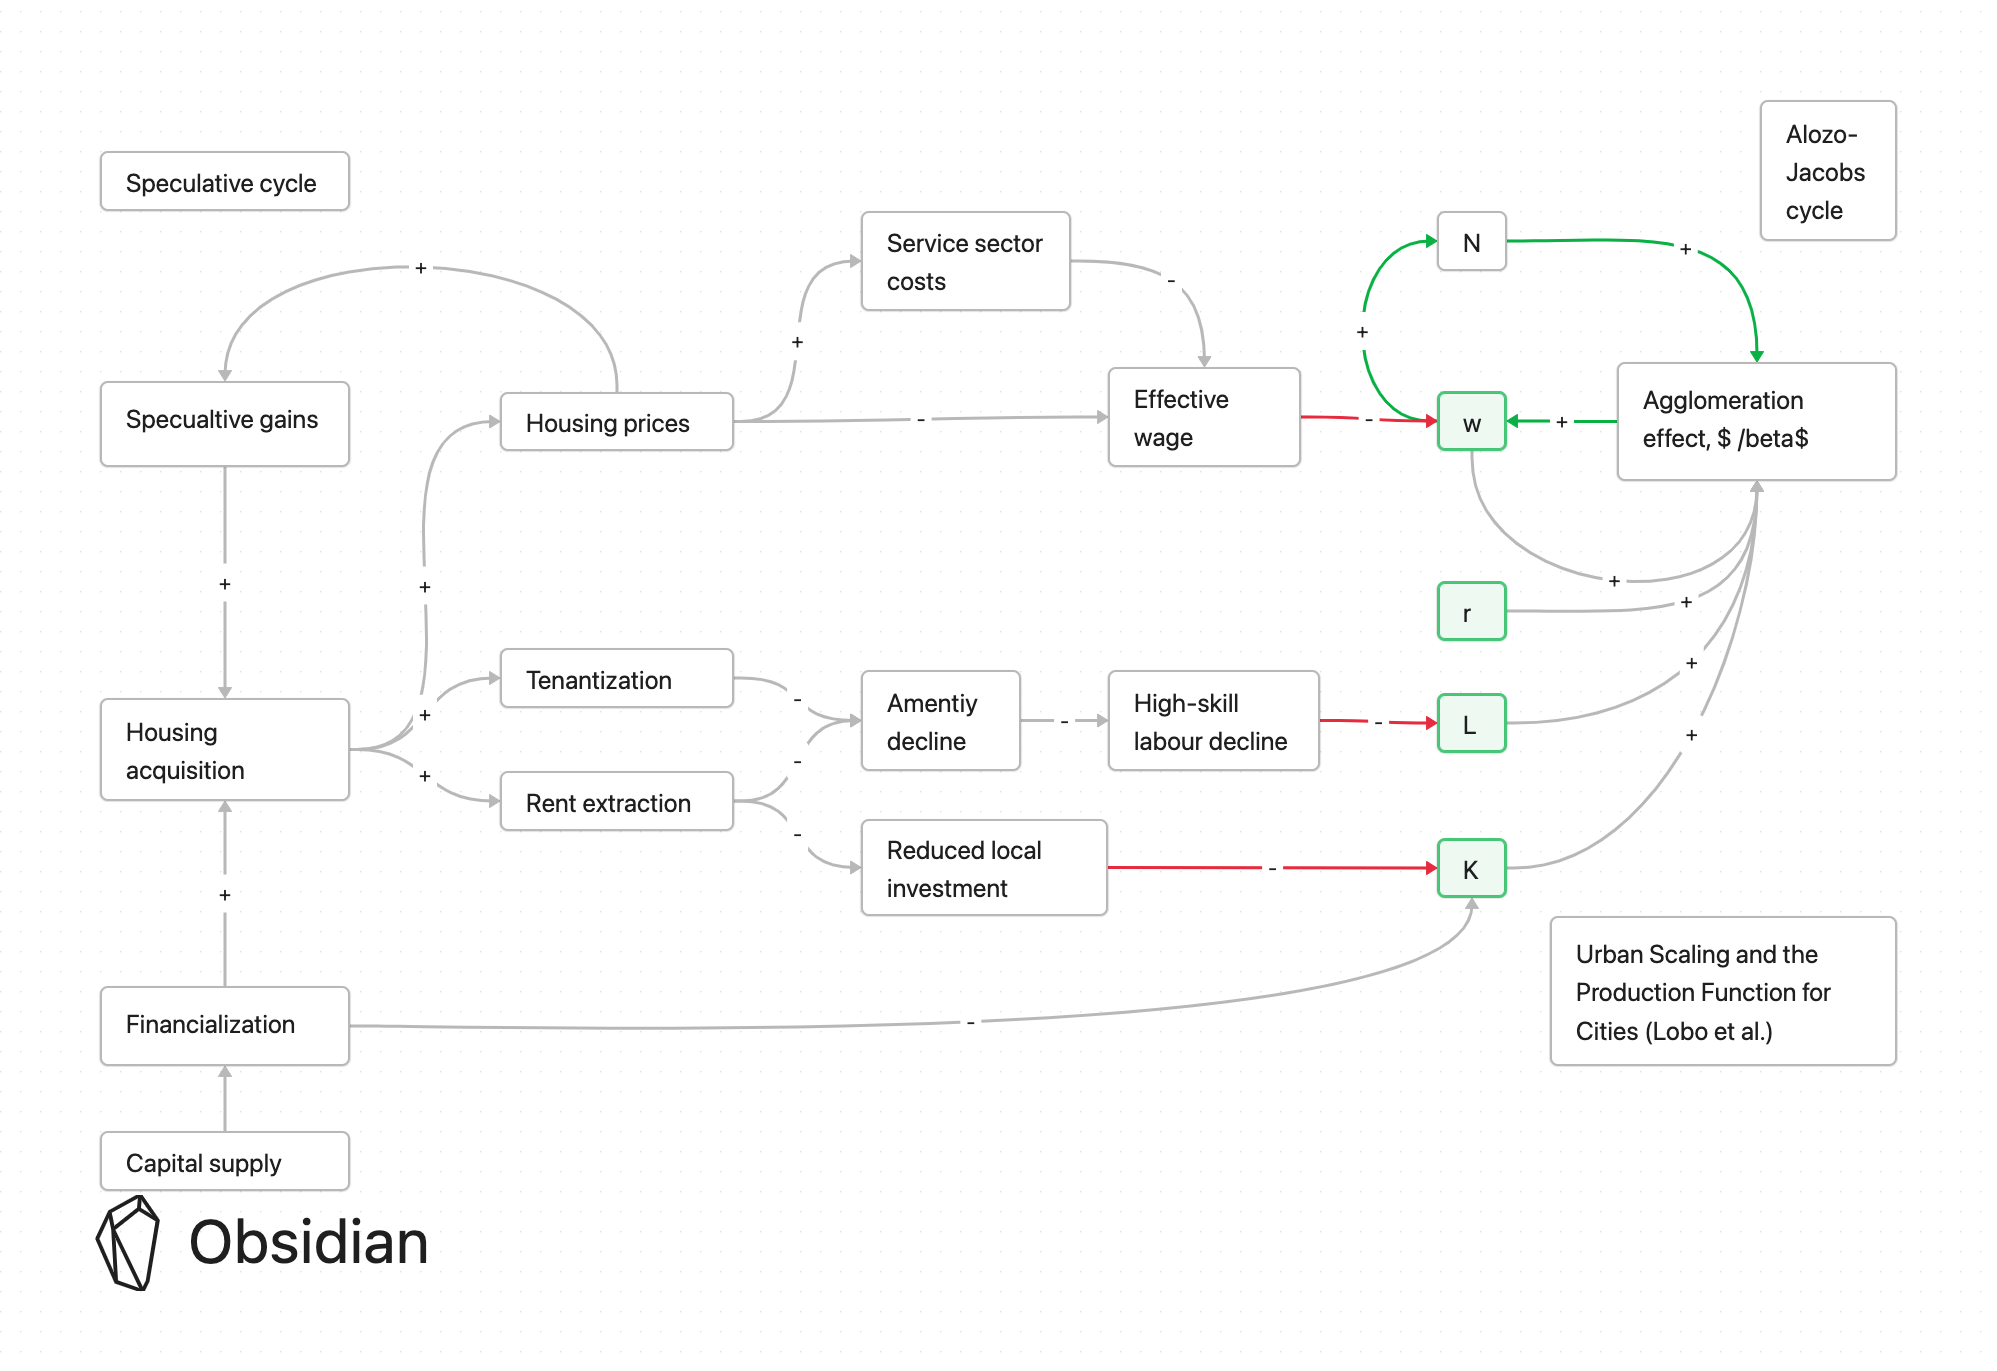
\includegraphics[scale=.25, angle=90]{fig/impact_channels.png}
%  \includegraphics[scale=.4, angle=90]%, angle=90
%    {fig/impact_channels_revised.png}
%     \label{fig-impact-ch}
% \caption[]{Impact channels of financialization}\label{fig-impact-channels}
% \end{figure}


 In Figure~\ref{fig-impact-channels} we illustrate how this argument relates to financialization. On the right are the variables that  Lobo et al \cite{loboUrbanScalingProduction2013} argue feed directly into determining $\beta$, which then sets the magnitude of the \gls{Alonzo-Jacobs cycle} at the top right.\footnote{This can be seen as modifying  the parameter in  the difference equation linking population to wage.} This is a relatively slow cycle. On the left in Figure~\ref{figure-impact-channels} is the self-reinforcing financialization-price increase- speculative  gain-financialization cycle. This is by comparison a very rapid cycle. Between the two cycles are the fine-grained differences between cities that actually explain the residuals in the estimates for specific cities. These finer features are, we suspect, historically determined and highly variable.

Glaeser and Saiz \cite{glaeserRiseSkilledCity2003} find little evidence for population growth accompanying skill upgrading among growing cities,  but they did find  evidence for skill upgrading that would increase effective labour in declining cities. Their results strongly  support the hypothesis of city-specific  and history-specific transmission from left to right in our figure.   

We can question whether the two-factor model in Lobo et al is an adequate representation. Neoclassical growth models incorporate human capital, which is itself a complex of technical knowledge, learned  skill and social capital. In other words  the neoclassical models can be seen as incorporating multiple factors conceptually while   suppressing them notationally. Similarly classical models  include land and resources explicitly while the two-factor model suppresses them.  These simplifications have been tremendously productive, in part because they allow us to focus on the large-scale and common features of the  system.  

The intermediate channels of impact we are attempting to tease out  in in this chapter and that appear in the empirical work as mere residuals might be understood as factors that have been suppressed because they are simply too fine-grained to deal with at this stage.
% on the right side we have variables that introduce the variation in beta for individual cities, which means that for any particular case, all the stuff in the middle is for a particular city.

% Over on the left we have the financialization, price increase, speculation cycle, its another self reinforcing city when it kicks in it feeds in through the dynamic of a particular city to affect the city
% but the mechanism in between is not a coarse grained one, it's a fine-grained one for each city.


We will begin with effects that work through the factor supply channels suggested by Lobo et al. 


\section{Influences on the scale parameter}

 
\begin{enumerate}
    \item financialization may make less local capital available and raises the cost of capital in the city. 
    
\item since rising rents reduce disposable income, inflation coming from the right  side of the figure will reduce  the effective urban wage, which Lobo et al find is one of the determinants of growth.

\item rent capture might influence the concentration of educated personnel by reducing the diversity and amenity of citries, making urban living less attractive 

\item rent capture leading to reduced local capital of reinvestment in human capital  might reduce the adaptive capacity of a city's population.

\item Rising housing costs might make it more difficult to attract or hold people with the specific adaptive skills Glaeser and Saiz identified.

\item  Rising housing costs would tend to squeeze low-wage workers out of the city, reducing the opportunity for upgrading the urban human capital efficiently. Glaeser and Saiz found   evidence for skill upgrading  in declining cities, which suggests efficient investment in less skilled workers. 

\item Rising housing costs at the centre of a city would tend to push low wage workers to the edges, increasing their transportation costs, putting further upward pressure on while increasing the costs of all amenity services that rely on lower-cost workers.

\item General financialization may have reduced the bargaining power of labor, as Tomaskovic-Devey and Lin  argue\cite{tomaskovic-deveyFinancializationCausesInequality2013}, reducing wages.\footnote{They point to a shift in behaviour of non-finance firms away from production and non-financial services and toward financial investments and services. This shift, they  argue,  has and led to lower employment, income transfers to executives and capital owners, and increased inequality among workers.\cite{tomaskovic-deveyFinancializationCausesInequality2013}}  

\end{enumerate}



Widening the discussion of channels, Duranton and Puga \cite{durantonMicroFoundationsUrbanAgglomeration2004} observee[] that ``Urban agglomeration economies are commonly classified into those arising from labour market interactions, from linkages between intermediate- and final-goods suppliers, and from knowledge spill-overs, loosely following the three main examples provided by Marshall (1890) in his discussion of the sources of agglomeration economies''  They go on to offer an alternative based on three types of micro-foundations for agglomeration, based on sharing, matching, and learning mechanisms. For this chapter we would like to identify any way that  financialization might affect one or more of these processes 

For Duranton and Puga, sharing gains arise because a larger final-goods industry will support a larger pool of input supplier who are able to offer the gains form specialization. This is an applications of one of Adam Smith's main insights. It is not obvious that financialization will significantly affect the scale of industry, or the number of suppliers.   One possible mechanism is that increasing costs and rising inequality might limit the diversity of consumption choices which functions as a component of the effective urban wage. Increasing costs and rising inequality might also limit the diversity of the labour pool, reducing the potential gains from specialization. Duranton and Puga  demonstrate that specialization by workers can generate increasing returns. It follows that any force that reduces the diversity of the workforce could eventually reduce $\beta$.  These channels are incorporated in Figure~\ref{fig-impact-channels}.

Matching mechanisms create increasing returns by cutting search costs for producers and by increasing the quality of matches. As the workforce grows and the number of firms increases the average worker is able to find an employer that is a better match for its skill. 

learning mechanisms




Glaeser and Saiz \cite{glaeserRiseSkilledCity2003} considered three explanations for why people increasingly crowd around the most skilled:  
\begin {enumerate} 
\item cities are increasingly oriented around consumption amenities, and skilled neighbors are an attractive consumption amenity. This suggests an effect on amenity or on the effective wage which can be defined as  including the  amenities of urban life. 
\item  cities exist to facilitate the flow of ideas and the skilled specialize in ideas. This suggests that for financialzation to have an effect it must reduce inhibit the networking capacity of  the city resulting in less effective labour being available.
\item cities survive only by adapting their economies to new technologies and human capital enables people to adapt well to change. 
\end{enumerate}
Their evidence shows that human capital only matters in potentially declining places, which  supports the third hypothesis: skills are valuable because they help cities adapt  to negative economic shocks.

Based on this kind of research, we should expect that cities with universities will grow more quickly and that financialization might have either positive or negative effects on the growth of local colleges and universities. 

\subsection{Effects through innovation}

%Belderbwhich ideas How quickly trom person to person.  %%% ???


Jacobs (1969, 1984) argued that interactions between people in cities help them get ideas and innovate, a view of cities that fits nicely with the work (Romer 1986; Lucas 1988)on economic growth that views externalities  externalities associated with knowledge spillovers as driving growth. Griliches (1979) surveyed the empirical literature on the role of knowledge spillovers. 

Three theories have dominated the discussion. The Marshall-Arrow-Romer (MAR) theory concerns knowledge spillovers between firms in an industry.  Marshall (1890) described how the concentration of an industry in a city helps knowledge
spillovers between firms and, therefore, the growth of that industry and of that city. Porter (1990) argued that local competition in concentration of industry drive innovation and growth. Both assume that technological spillovers occur within a=n industry. In the Jacobs-Rosenberg\cite{rosenbergTechnologicalChangeMachine1963}-Bairoch \cite{bairochCitiesEconomicDevelopment1988} model,\footnote{Glaeser et al \cite{glaeserGrowthCities1991} refer to the Jacobs model as the Jacobs-Rosenberg\cite{rosenbergTechnologicalChangeMachine1963}-Bairoch \cite{bairochCitiesEconomicDevelopment1988} model. } unlike MAR and Porter, believes that the most important knowledge transfers come from outside the core industry through cross-fertilization among a variety  of  industries.

%Bairoch, P. (1988)\cite{Condit1990CitiesAE}. Cities and Economic Development: From the Dawn of History to the Present. Chicago, IL: University of Chicago Press.

Scherer (1982) presented systematic evidence indicating that around 70 percent of inventions in a given industry are used outside that industry. Much evidence thus suggests that knowledge spills over across industries. Because cities bring together people from different walks of life, they foster transmission of ideas.


Glaeser, Kallal, Sheinkman and Shleifer \cite{glaeserGrowthCities1991} used data on 170 of the largest US cities which industries in which cities grew fastest between 1956 and 1987 and why. They found that  industries grow slower in cities in which
they are more heavily over-represented and faster where the firms in the industry are smaller than the national average  and when the city is less specialized. This evidence is
thus negative on MAR, mixed on Porter, and consistent with Jacobs.

Henderson 1986 presented evidence that output per labour hour is higher i when firms in the same industry are clustered.

Henderson also described "urbanization externalities" that lead different firms to locate together. In this view urbanization increases final market demand and diveristy of products, but Glaeser et al suggest that this effect does not drive growth

Lobos et. al examine the simultaneous effects of spillovers due to research and development by universities and by firms \cite{belderbosWhatSpilloversUniversities2022}.

Glaeser et al \cite{glaeserGrowthCities1991} tested a model  of employment growth (not productivity growth) in an industry in a city as a function of the specialization of that industry in that city, local competition in the city-industry, and city diversity. None of the their results  support the importance
of within-industry knowledge spillovers for growth. If such spillovers. %This may be usefull for us because it rules out a veryd ifficult channel to examine.
\section{Network accounts}
Network accounts of increasing returns have drawn a good deal of attention.
Johansson and Quigley \cite{johanssonAgglomerationNetworksSpatial} in \cite{floraxFiftyYearsRegional2004} consider the parallel developments in the economics of agglomeration and the economics of networks, making a distinction between public and private capital in generating efficiencies.

\begin{quotation}
"the formation and efficiency of agglomeration arise from its character as public capital; households and firms in the same agglomeration share its benefits in common. In contrast, an economic network is private capital shared primarily by the network participants. Agglomerations also rely on public institutions, which aggregate individual decisions. In contrast, economic networks arise from a collective decision by group members, generating a private institution. Networks are clubs in which exclusion is possible and price discrimination is the norm. Agglomerations cannot exclude economic actors from receiving benefits nor can they price these benefits efficiently."
\end{quotation}
They point out, drawing on Dixit and Stiglitz \cite{AvinashK.Dixit1977MCaO},  Fujita \cite{fujitaMonopolisticCompetitionModel1988}, Stiglitz and Venables and \cite{fujitaSpatialEconomyCities1999} that economies of scale  can arise with the diversification of the consumer market or of the input market, even though all individual competitors and firms earn normal profits. In such cases, it is not necessary for firms to internalize the effects of increasing their workforce, because they enjoy growing external economies.

 It is a remarkable result, but can the financialization of the housing market affect this class of  gains? It would appear unlikely unless the changing population mix induced by financialization led to a thinning of the local market for consumer goods. 

 The second mechanism they identify is at the firm level and forward and backward linkages among agents. These linkages may be of a pure-market type or may involve transaction links. They yield  gains from proximity or localization rather than urbanization specifically, although urbanization may be the force leading to localization. Can the financialization of the housing market affect this class of  gains? One feature of financialization has been the acquisition of firms, in many cases followed by layoffs, management changes, and consolidations focused on rapid profits and stock gains. Arguably these changes can inhibit urban growth but these effects are unrelated to the housing market.
 

\section{Effects through inequality}
Barro \cite{barroInequalityGrowthInvestment1999} found that inequality had a negative effect on growth in poorer countries but no significant effect for the richer countries. Grigoli et al \cite{grigoliInequalityGrowthHeterogeneous2016} find  that the effect of income inequality on economic growth can be either positive or negative, and that at levels  of inequality  represented by a Gini coefficient below about 27  to be exact inequality hurts economic development. \footnote{Canada's Gini Coefficient Index was 66.7 in 2017. } %PUZZLE

 ``On the one hand, a higher concentration of income in the hands of a few is reflected in reduced demand by a larger share of poorer individuals, which would invest less in education and health and grow a sense of social and political discontent, jeopardizing human capital and stability. Moreover, more inequality can exacerbate households’ leverage to compensate for the erosion in relative income, empower the influence of the richer population on the legislative and regulatory processes, and motivate redistribution policies that are often blamed for slowing growth, especially when aggressive. On the other hand, a certain level of inequality endows the richer population with the means to start businesses, as well as creates incentives for individuals to increase their productivity and invest their saving, hence promoting economic growth.';'Across income levels, only the findings for emerging markets indicate that more inequality slows economic growth. The only country groups for which we find evidence of a significant negative effect are the Middle East and Central Asia, the Western Hemisphere, and emerging markets (3/8).

 But Canada is in the western hemisphere, with inequality more like that of ERurope 
 
 Other theories propose a positive relationship. These are based on the argument that inequality can rather provide incentives for innovation and higher productivity (Lazear and Rosen, 1981; Okun, 2015), foster saving and investment to the extent that rich people have a higher propensity to save (Kaldor, 1957), and endow richer individuals with the minimum capital and education needed to start some economic activity (Barro, 2000)
Bivens, reporting on the USA, argues that inequality is reducing growth by reducing the aggregate demand of the population below the 90$^{th}$ percentile in income.\cite{bivensInequalitySlowingUS2017} 



----


% The notion that your labour force is on average more productive when there are more people around is pretty dramatic and it's very much not part of the basic model that we use. Our starting point is that's the fundamental feature of cities, and what does that do with financial capital and what does that do to distribution and that's not been explored. 

% The concentration of wealth is associated with slower econ growth.  There's a possibility that somehow the city will grow less.
% %{\color{red} We can speculate on how the distribution. of wealth directly affects the scaling parameter $\beta$. This probably calls of a discussion of the paths through which agglomeration works } 


\subsection{Spillovers}
Belderbos et. al examine the simultaneous effects of spillovers due to research and development by universities and by firms \cite{belderbosWhatSpilloversUniversities2022}. Rising urban productivity in Japan are significant. 




% \subsection{Financialization and productivity}

% For urban theory and policy formation it is important to distinguish between financial instruments that enable production of real assets, and instruments like  mortgages that primarily facilitate the transfer of real assets or rights to real estate income. Housing developers borrow to purchase land for development and builders borrow to finance construction. While important, the financial instruments involved are not driving the financialization of housing.  The size of the loans involved is affected by the amount of land purchased and the potential rents earned by that land, but the degree of non-occupant ownership is not affected. *** CLARIFY

% Although inflows of financing through financialization, can fund development, financialization of the does not add to the housing stock in it's own right. Financialization refers the process of transferring ownership of existing housing units. 

% When  a productive asset is acquired as a financial asset it remains productive.  The financial instrument is separate form the real asset, at least in principle, and is traded in different markets. Why then is financialization an issue?  Theory suggests that financialization is positive.  The major argument is that finacialization enables real investment. In theory then, financialization of the housing market therefore  to more housing production. It is striking that after 40 years of growing financialization across we face a housing crisis , increasing homelessness and falling rates of home ownership.  Palley \cite{palleyFinancializationWhatIt2007} says that 

% \begin{quotation}At the macroeconomic level the era of financialization has been associated with generally tepid economic growth.\dots  In all countries except the U.K., average annual growth fell during the era of financialization that set in after 1979. Additionally, growth also appears to show a slowing trend so that growth in the 1980s was higher than in the 1990s, which in turn was higher than in the 2000s. \end{quotation}

% African land or land in Northern Ontario 
% Land acquired by holding companies may even be made more productive. The theory is that 
% the goal of such investments, however, is generally to achieve a capital gain over time. Financial analysis is essentially about rates of return on financial capital invested. The opportunity for capital gains  attracts financial capital to the housing market.%Financial managers have no interest is n in assets that are not expected to increase in value. 

% ***ILLUSTRATE AND CLARIFY
% If you see it as just supply and demand .. 
% Supply demand with fixed product and everything’s neat
% Agglomeration changes everything. firms are underestimating each time they add a worker, the value that’s going to be produced. They benefit from an agglomeration effect and that’s where they interesting dynamics are coming from..
% we know that there is a marginal product of labour for a firm that it should be able to figure it out.. can the person on the shop floor figure out whether it's worth hiring another person.. we can talk about it, add details etc. We have a declining marginal product of labour. Because of transportation costs, we have a rising cost of getting labour so they cross and there is an equilibrium. There are adjustment questions like which adjusts quickly, how fast people move in, how fast firms decide to hire etc, but we know that there is in principle and equilibrium and that it is in principle a stable equilibrium (DIAGRAM STROGATS) although there are complications with this-- some argue these market equilibria never make sense- true in lots of way, but useful for analysis. 
% The question is then, what happens in our city? Do you get a growth dynamic? What seems to be the case is that if all the firms add workers then the marginal value of the product of all the workers they have goes up, which means they are making more profit which means if they are making more profit they want to hire more workers? Does it ever converge? Likely eventually, but it's got a very powerful dynamic.  If you add other features like more products being created in the city, which is part of this agglomeration process you can start seeing, if you exhaust one source of growth, we know that there are others, that simplification is just firms of the same sort hiring workers of the same sort is wrong. so we need to add the local service sector, we need to add the possibility of creating new products and those depends on the number of workers and so depend on further agglomeration effects. What does this mean? For the purpose of the model, we'd want to strengthen the agglomeration effect relative to what they are for specific firms or industries..



MOVE?  YES

 Notice that this formulation implies it is possible to have increasing returns to scale for the urban economy even with a production function at the firm level with decreasing returns to scale: the return to the total economy $\alpha + \beta(1 + \gamma)$ can be greater than one, even if $\alpha +\beta$ is less than one. %.\label{Fn:PSI}}  (CITE Appendix: Excess Returns)
 
The \gls{agglomeration effect} means that although individual firm returns to scale are declining, the city can experience \gls{increasing returns to scale} in the utilization of human capital. % NEED? Individual firms have decreasing returns, but the presence of agglomeration economies external to firms but internal to the city gives the urban economy as a whole increasing returns to scale .}.
%\footnote{The formulation is consistent with the discussion of endogenous growth theory in Chapter \ref{chapter-growth}, which demonstrated that increasing returns at the macro level is consistent with decreasing returns at the micro level. The effects are not limited to the individual firm. \Gls{spillover effects} can be large, see section \ref{section-spillover}. }






\begin{quotation}`` high productivity cities show invariably high wages and high levels of employment relative to their size expectation. Conversely, low productivity cities show both low wages and employment.''

\dots Urbanization and growth go together: no country has ever reached middle- income status without a significant population shift into cities \cite{annezUrbanizationGrowthSetting2009}\end{quotation}




%\cite{rosenthalEvidenceNatureSources2004}
This gives 
A language to talk about a whole class of problems that are important/of rising importance in the literature but that this class of formal models has lacked the infrastructure/language/conceptual toolkit to explore. ** MAYBE ALSO MENTION THIS IN DOC INTRO/CONCLUSION
NEED TO SHOW A CONNECTION BETWEEN GROWTH RATE AND DISTRIBUTION - IN THE GROWTH CHAPTER.. -- OR RIGHT AFTER AS A NEW CHAPTER..



\epigraph{Widespread urbanization is a recent phenomenon. In 1900 just 15 percent of the world’s population lived in cities. The 20th century transformed this picture, as the pace of urban population growth accelerated very rapidly in about 1950. Sixty years later, it is estimated that half of the world’s people lives in cities.}{Annez and Buckley\cite{annezUrbanizationGrowthSetting2009}}


****  Urban infrastructure has high social but low private returns. It is unlikely private capital will flow into urban infrastructure projects with substantial public support. That is the motive for ``\gls{Public-Private Partnerships}'' (PPPs) that involve private capital financing government projects and services up-front, and then subsidizing the private investors  from taxpayers out of the expected social returns over the course of the PPP
Annez and Buckley\cite{annezUrbanizationGrowthSetting2009} observe that 
\begin{quotation}
Britain’s cities were cleaned up only when the central government stepped in to alleviate the binding financial constraint in cities. In this story lies an important lesson about building urban infrastructure, especially those lumpy discrete investments in networks that expand the limits at which congestion costs outweigh agglomeration benefits. Neither the municipal finance systems that worked before the urban transition nor those suitable for cities in a demographic steady state will necessarily generate finance for investments in local public goods that more than pay for themselves in economic terms. 
\end{quotation}




%``As Quigley points out in chapter 4, the fundamental question in urban economics is why people voluntarily live in close proximity to one another when there are costs to competing for land. The simple answer has two parts: efficiency gains and consumption benefits. Recent theoretical and empirical work provides a sense of the nature and significance of these gains.'' Annez and Buckley\cite{annezUrbanizationGrowthSetting2009}% P  13 %see theie list



%Evidence from a broad panel of countries shows little overall relation between income inequality and rates of growth and investment. However, for growth, higher inequality tends to retard growth in poor countries and encourage growth in richer places. The Kuznets curve-whereby inequality first increases and later decreases during the process of economic development-emerges as a clear empirical regularity.


Policy tools unrelated to financialization can be examined in this  frame we use here. Cutting transportation costs in a city is equivalent to raising the effective wage, which would  make it easier to attract labour and reduce pressure on producers to raise wages. It would also reduce the cost of education for commuters, increasing the supply of augmented labour.



 We can mimic the effects of financialization as it works through reduction in the effective wage by introducing a gap between the value of the marginal product of labour and the wage paid. 

